\IfFileExists{figures/flow_performance.png}{%
\begin{figure}[H]
    \centering
    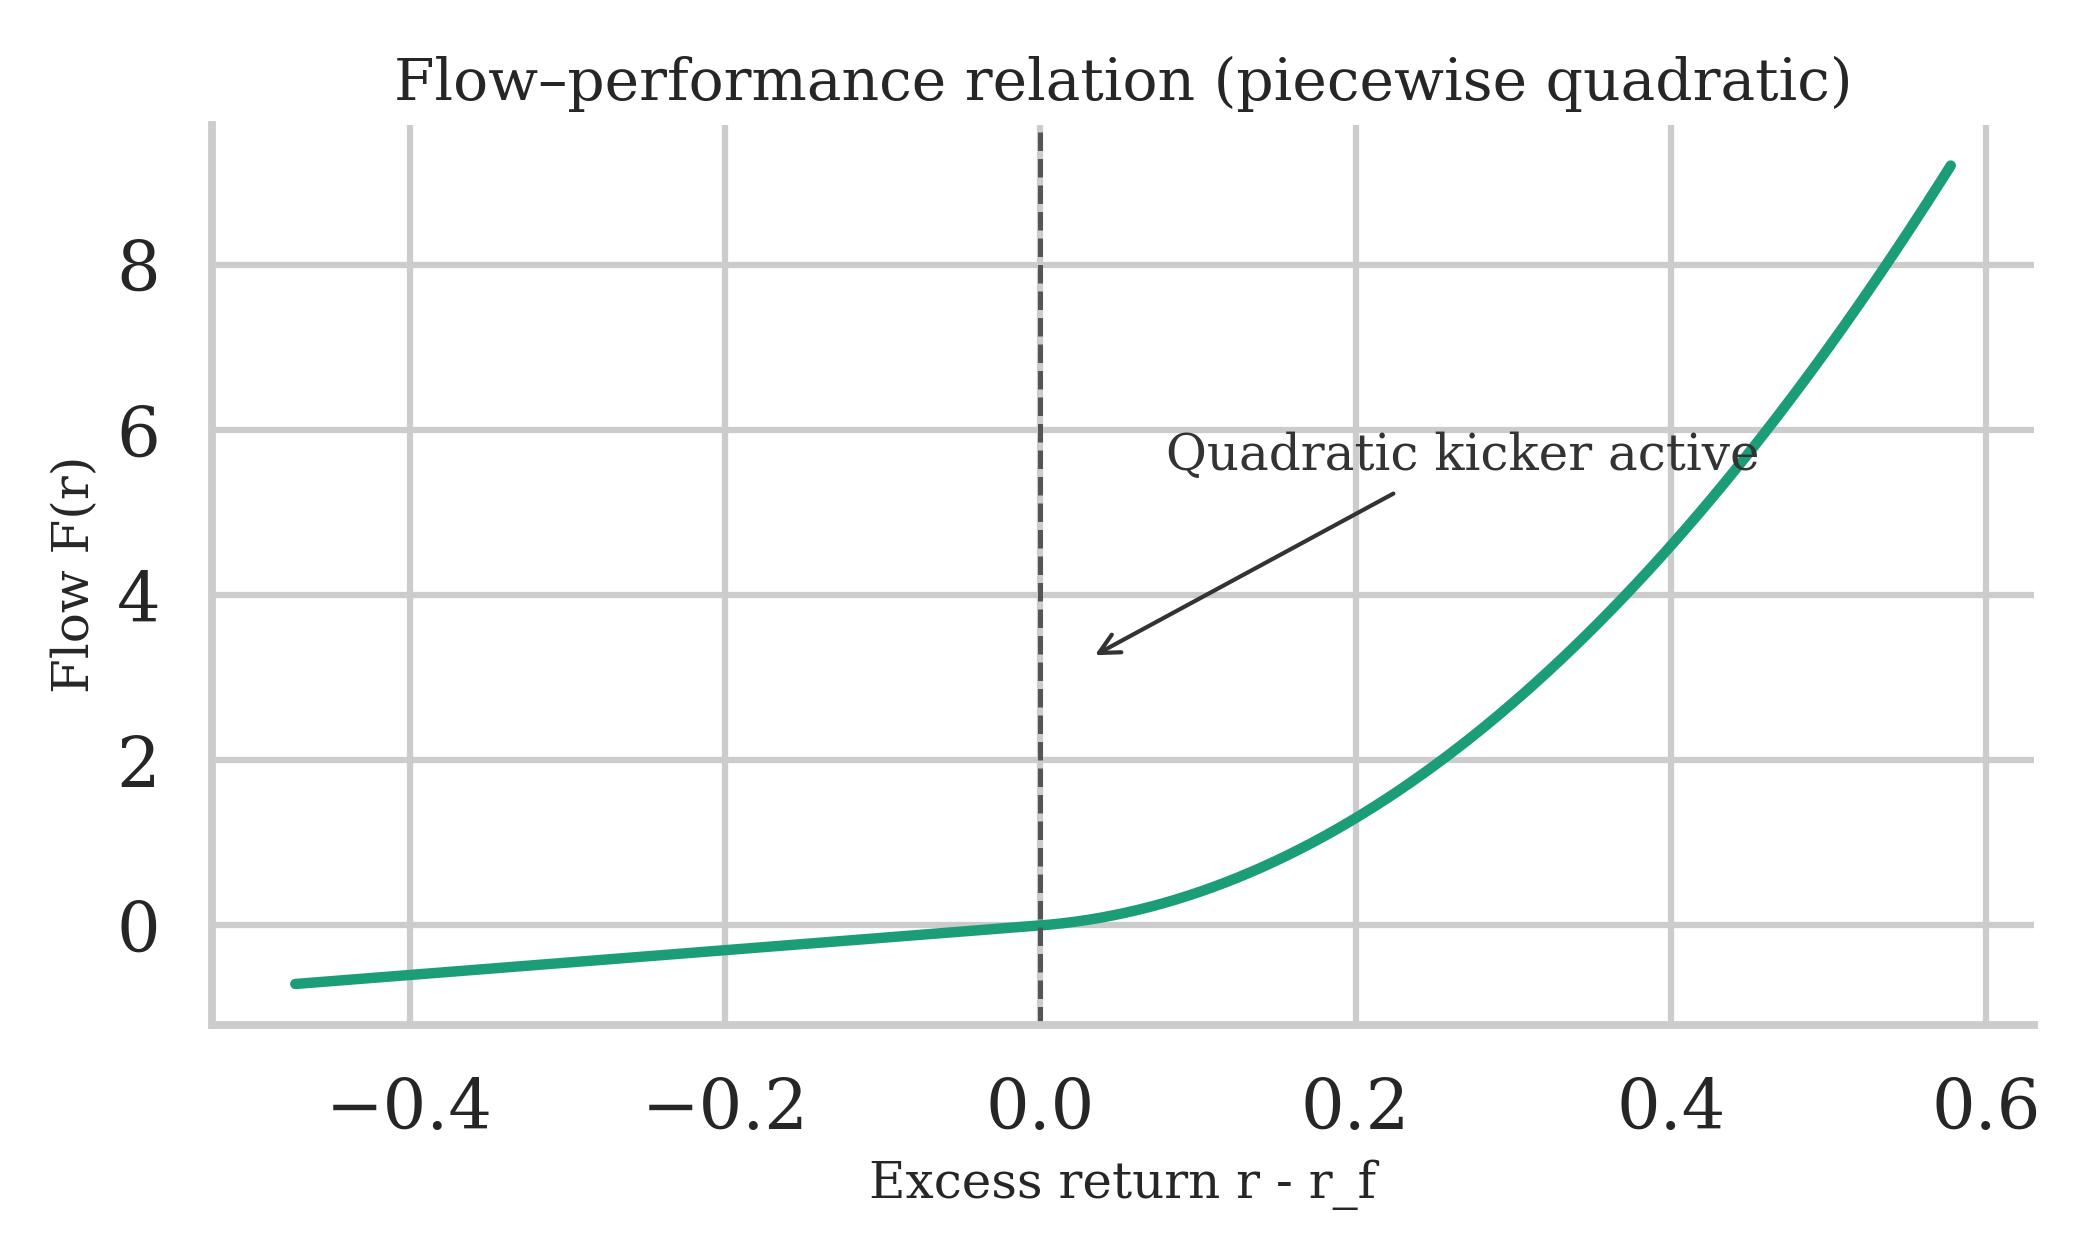
\includegraphics[width=0.85\linewidth]{figures/flow_performance.png}
    \caption{Flow–performance relation used in the model. The linear term applies in all states; a quadratic kicker activates once performance exceeds cash, capturing empirical convexity in flows \citep[][]{sirri1998costly, chevalier1997risk}.}
    \fnote{\textit{Note:} Calibrated baseline parameters: $\Sharpe=0.35$, $r_f=3.70\%$, $\gamma=5$, $\eta=15$, $A_0=1$, $f_1=1.5$, $f_2=25$. Illustration uses $\sigma=0.15$ for visual clarity.}
    \label{fig:flow-performance}
\end{figure}
}{}

\IfFileExists{figures/ic_fee_curve.png}{%
\begin{figure}[H]
    \centering
    
\includegraphics[width=0.85\linewidth]{figures/ic_fee_curve.png}
    \caption{Incentive–compatible fee \(\phi(\sigma_d)\) as a function of the target volatility \(\sigma_d\) under different flow convexities \(f_2\). Higher convexity reduces the fee required to discipline risk taking.}
    \fnote{\textit{Note:} Other parameters at calibration baseline: $\Sharpe=0.35$, $r_f=3.70\%$, $\gamma=5$, $\eta=15$, $A_0=1$, $f_1=1.5$. Four values of $f_2$ are shown: 5, 15, 25 (baseline), and 50.}
    \label{fig:ic-fee-curve}
\end{figure}
}{}

\IfFileExists{figures/opt_sigma_vs_f2.png}{%
\begin{figure}[H]
    \centering
    
\includegraphics[width=0.85\linewidth]{figures/opt_sigma_vs_f2.png}
    \caption{Optimal investor target volatility \(\sigma_d^*\) as a function of the convexity parameter \(f_2\). Stronger convexity lowers \(\sigma_d^*\), consistent with the comparative statics.}
    \fnote{\textit{Note:} Other parameters held at calibration baseline: $\Sharpe=0.35$, $r_f=3.70\%$, $\gamma=5$, $\eta=15$, $A_0=1$, $f_1=1.5$.}
    \label{fig:opt-sigma-vs-f2}
\end{figure}
}{}

\IfFileExists{figures/compstats_f2.png}{%
\begin{figure}[H]
    \centering
    
\includegraphics[width=0.95\linewidth]{figures/compstats_f2.png}
    \caption{Comparative statics with respect to convexity: optimal target \(\sigma_d^*\) and IC fee at the optimum \(\phi(\sigma_d^*)\) as functions of \(f_2\).}
    \fnote{\textit{Note:} Other parameters held at calibration baseline: $\Sharpe=0.35$, $r_f=3.70\%$, $\gamma=5$, $\eta=15$, $A_0=1$, $f_1=1.5$.}
    \label{fig:comp-f2}
\end{figure}
}{}

\IfFileExists{figures/compstats_scale.png}{%
\begin{figure}[H]
    \centering
    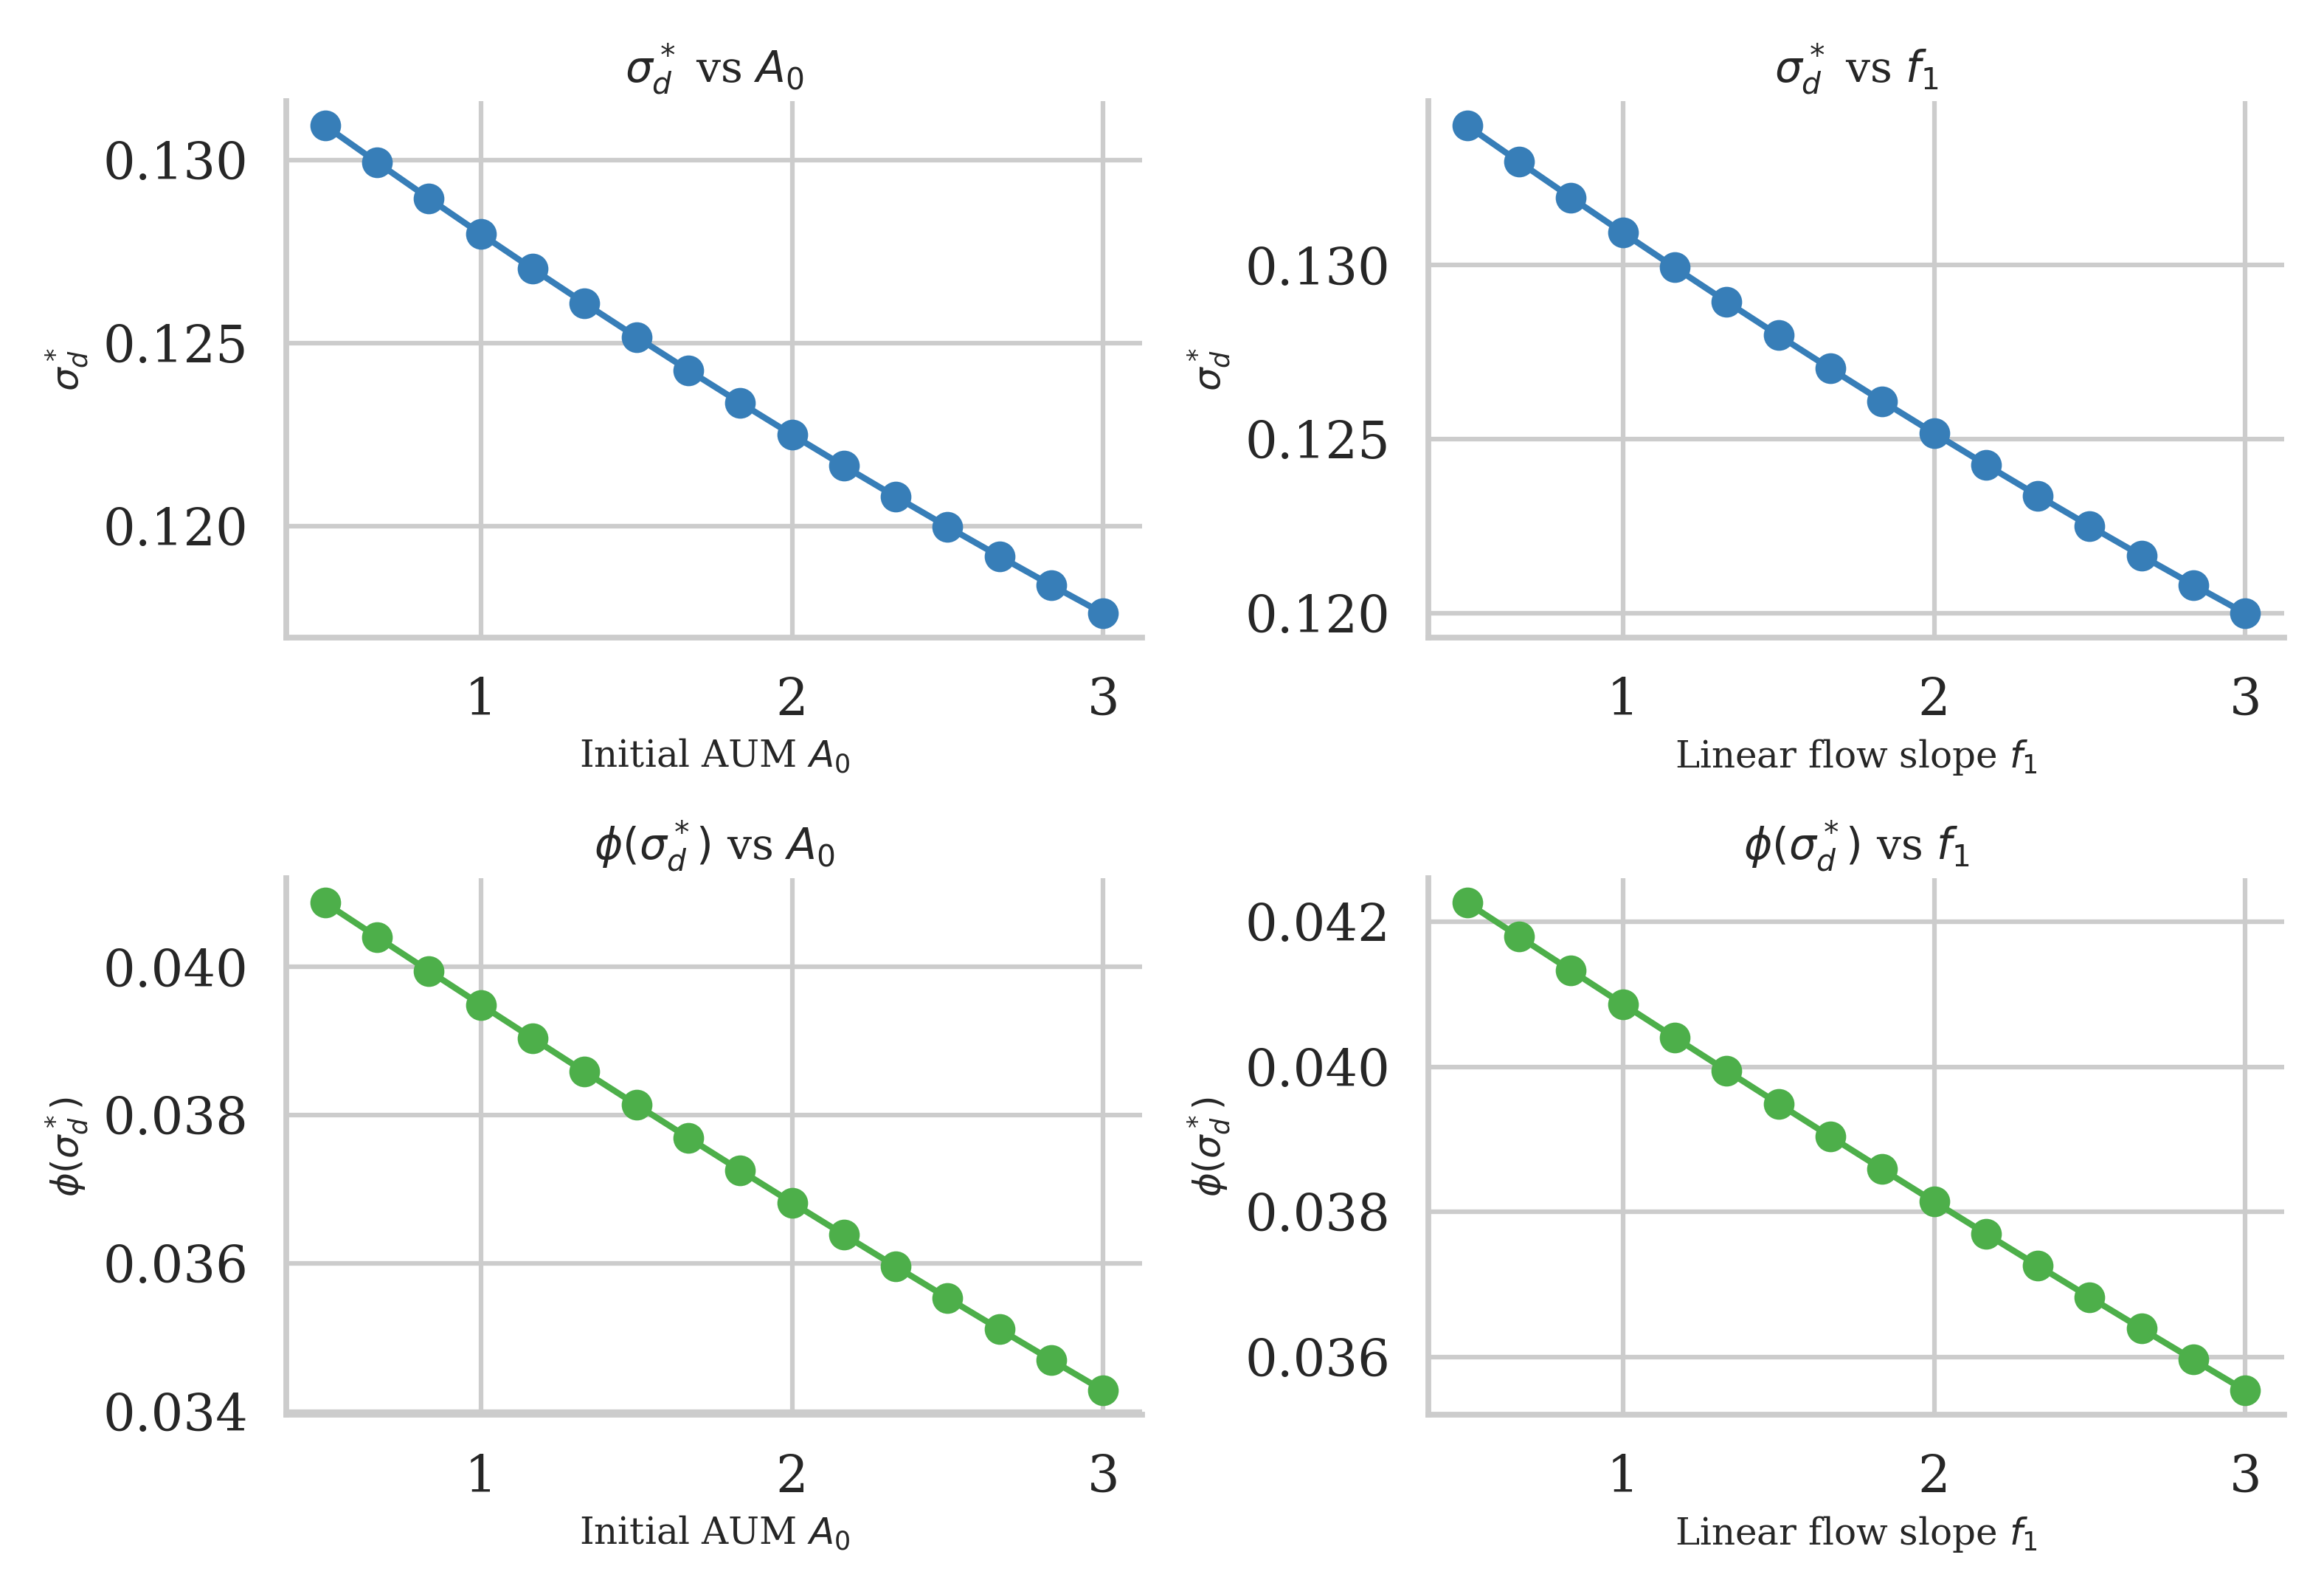
\includegraphics[width=0.95\linewidth]{figures/compstats_scale.png}
    \caption{Scale effects: optimal target \(\sigma_d^*\) and IC fee at the optimum \(\phi(\sigma_d^*)\) as functions of initial AUM \(A_0\) and the linear flow slope \(f_1\).}
    \fnote{\textit{Note:} Other parameters held at calibration baseline: $\Sharpe=0.35$, $r_f=3.70\%$, $\gamma=5$, $\eta=15$, $f_2=25$. Left panel varies $A_0$ with $f_1=1.5$; right panel varies $f_1$ with $A_0=1$.}
    \label{fig:comp-scale}
\end{figure}
}{}

\IfFileExists{figures/compstats_sharpe.png}{%
\begin{figure}[H]
    \centering
    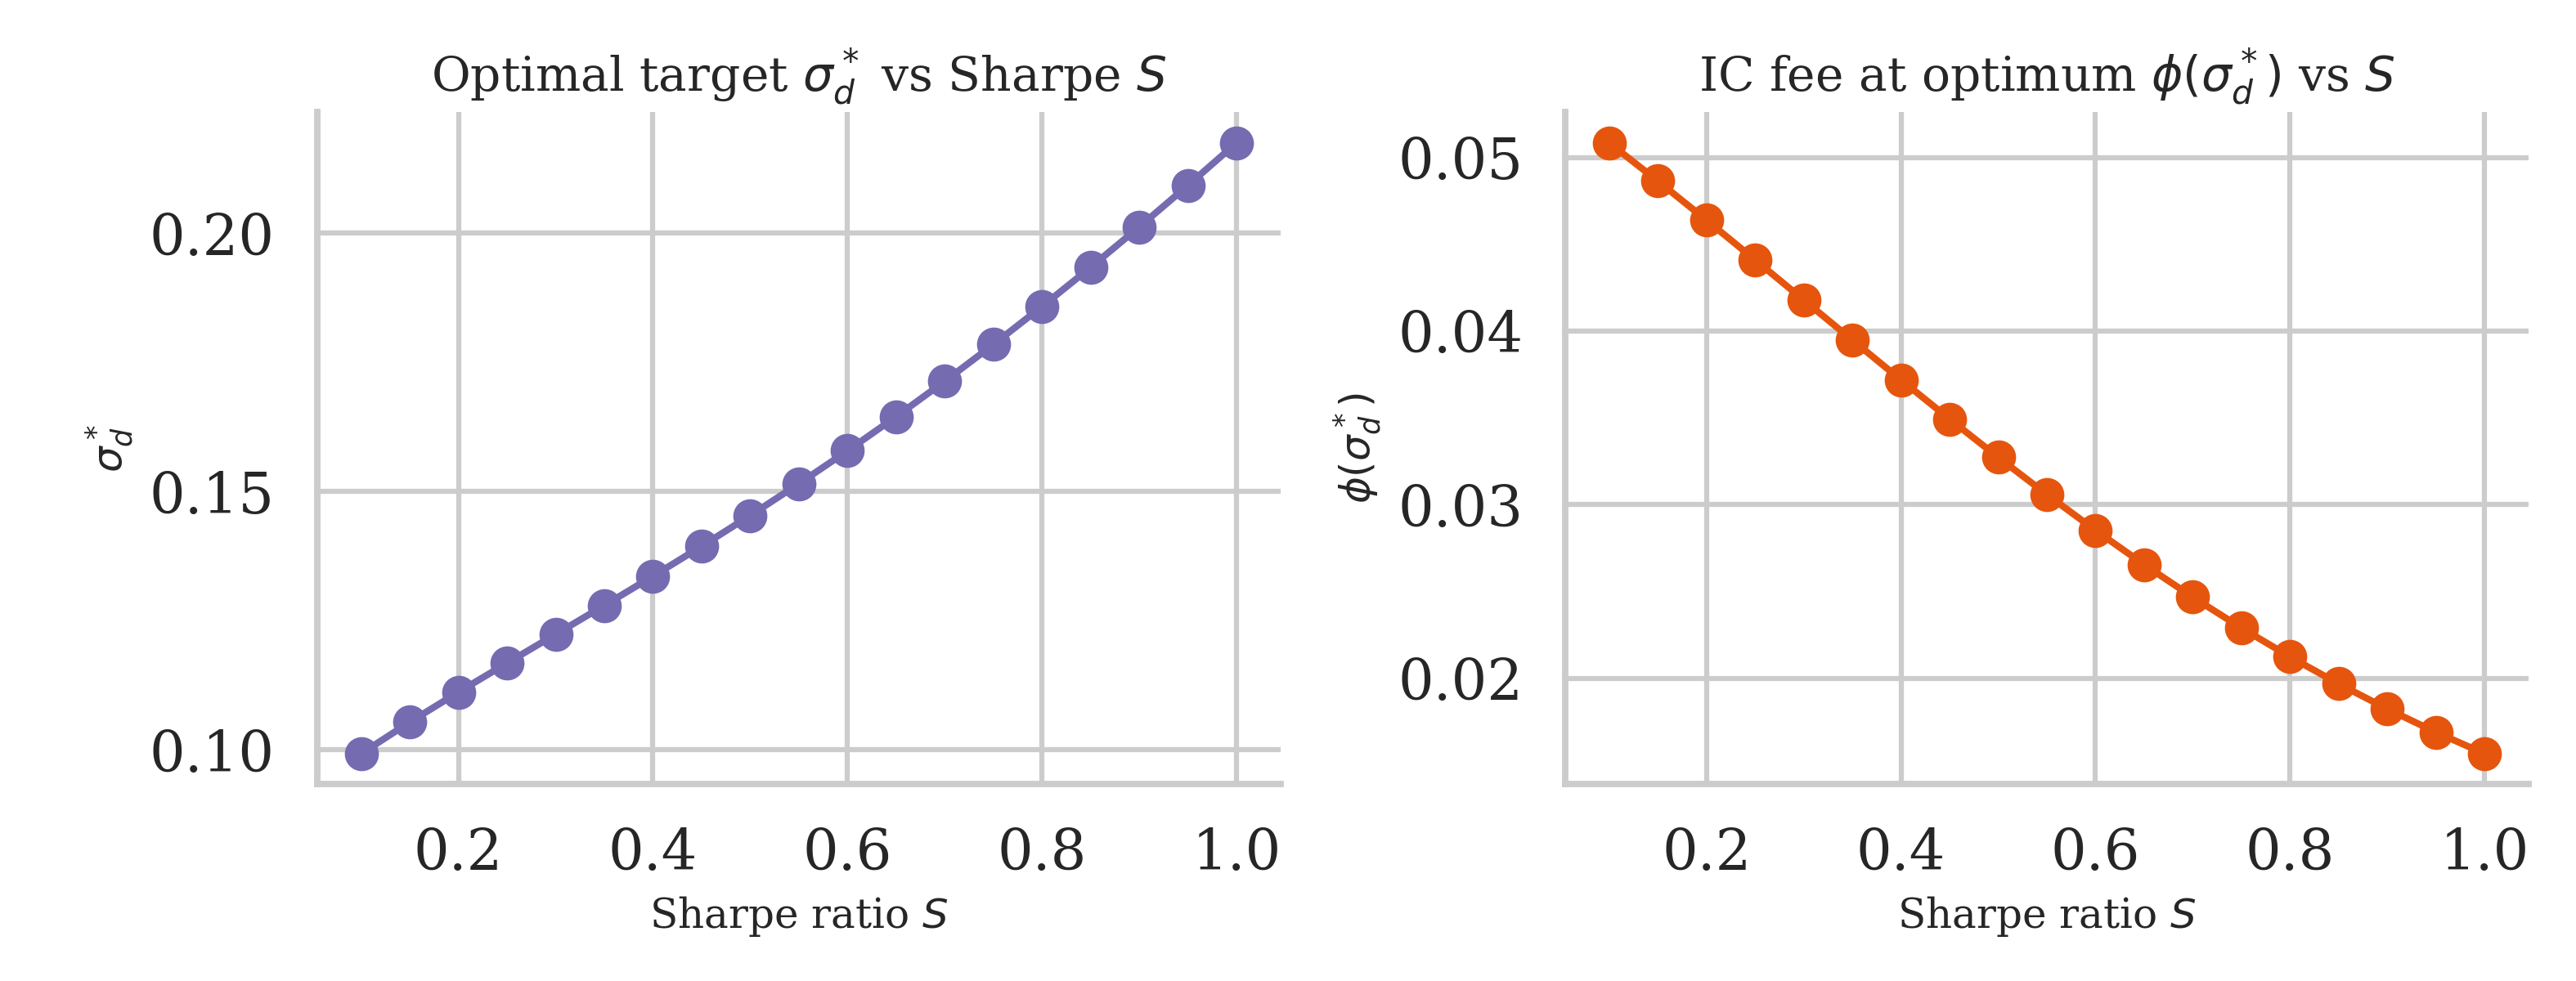
\includegraphics[width=0.95\linewidth]{figures/compstats_sharpe.png}
    \caption{Managerial skill effects: optimal target \(\sigma_d^*\) and IC fee at the optimum \(\phi(\sigma_d^*)\) as functions of the Sharpe ratio \(S\).}
    \fnote{\textit{Note:} Other parameters held at calibration baseline: $r_f=3.70\%$, $\gamma=5$, $\eta=15$, $A_0=1$, $f_1=1.5$, $f_2=25$.}
    \label{fig:comp-sharpe}
\end{figure}
}{}

\IfFileExists{figures/compstats_risk.png}{%
\begin{figure}[H]
    \centering
    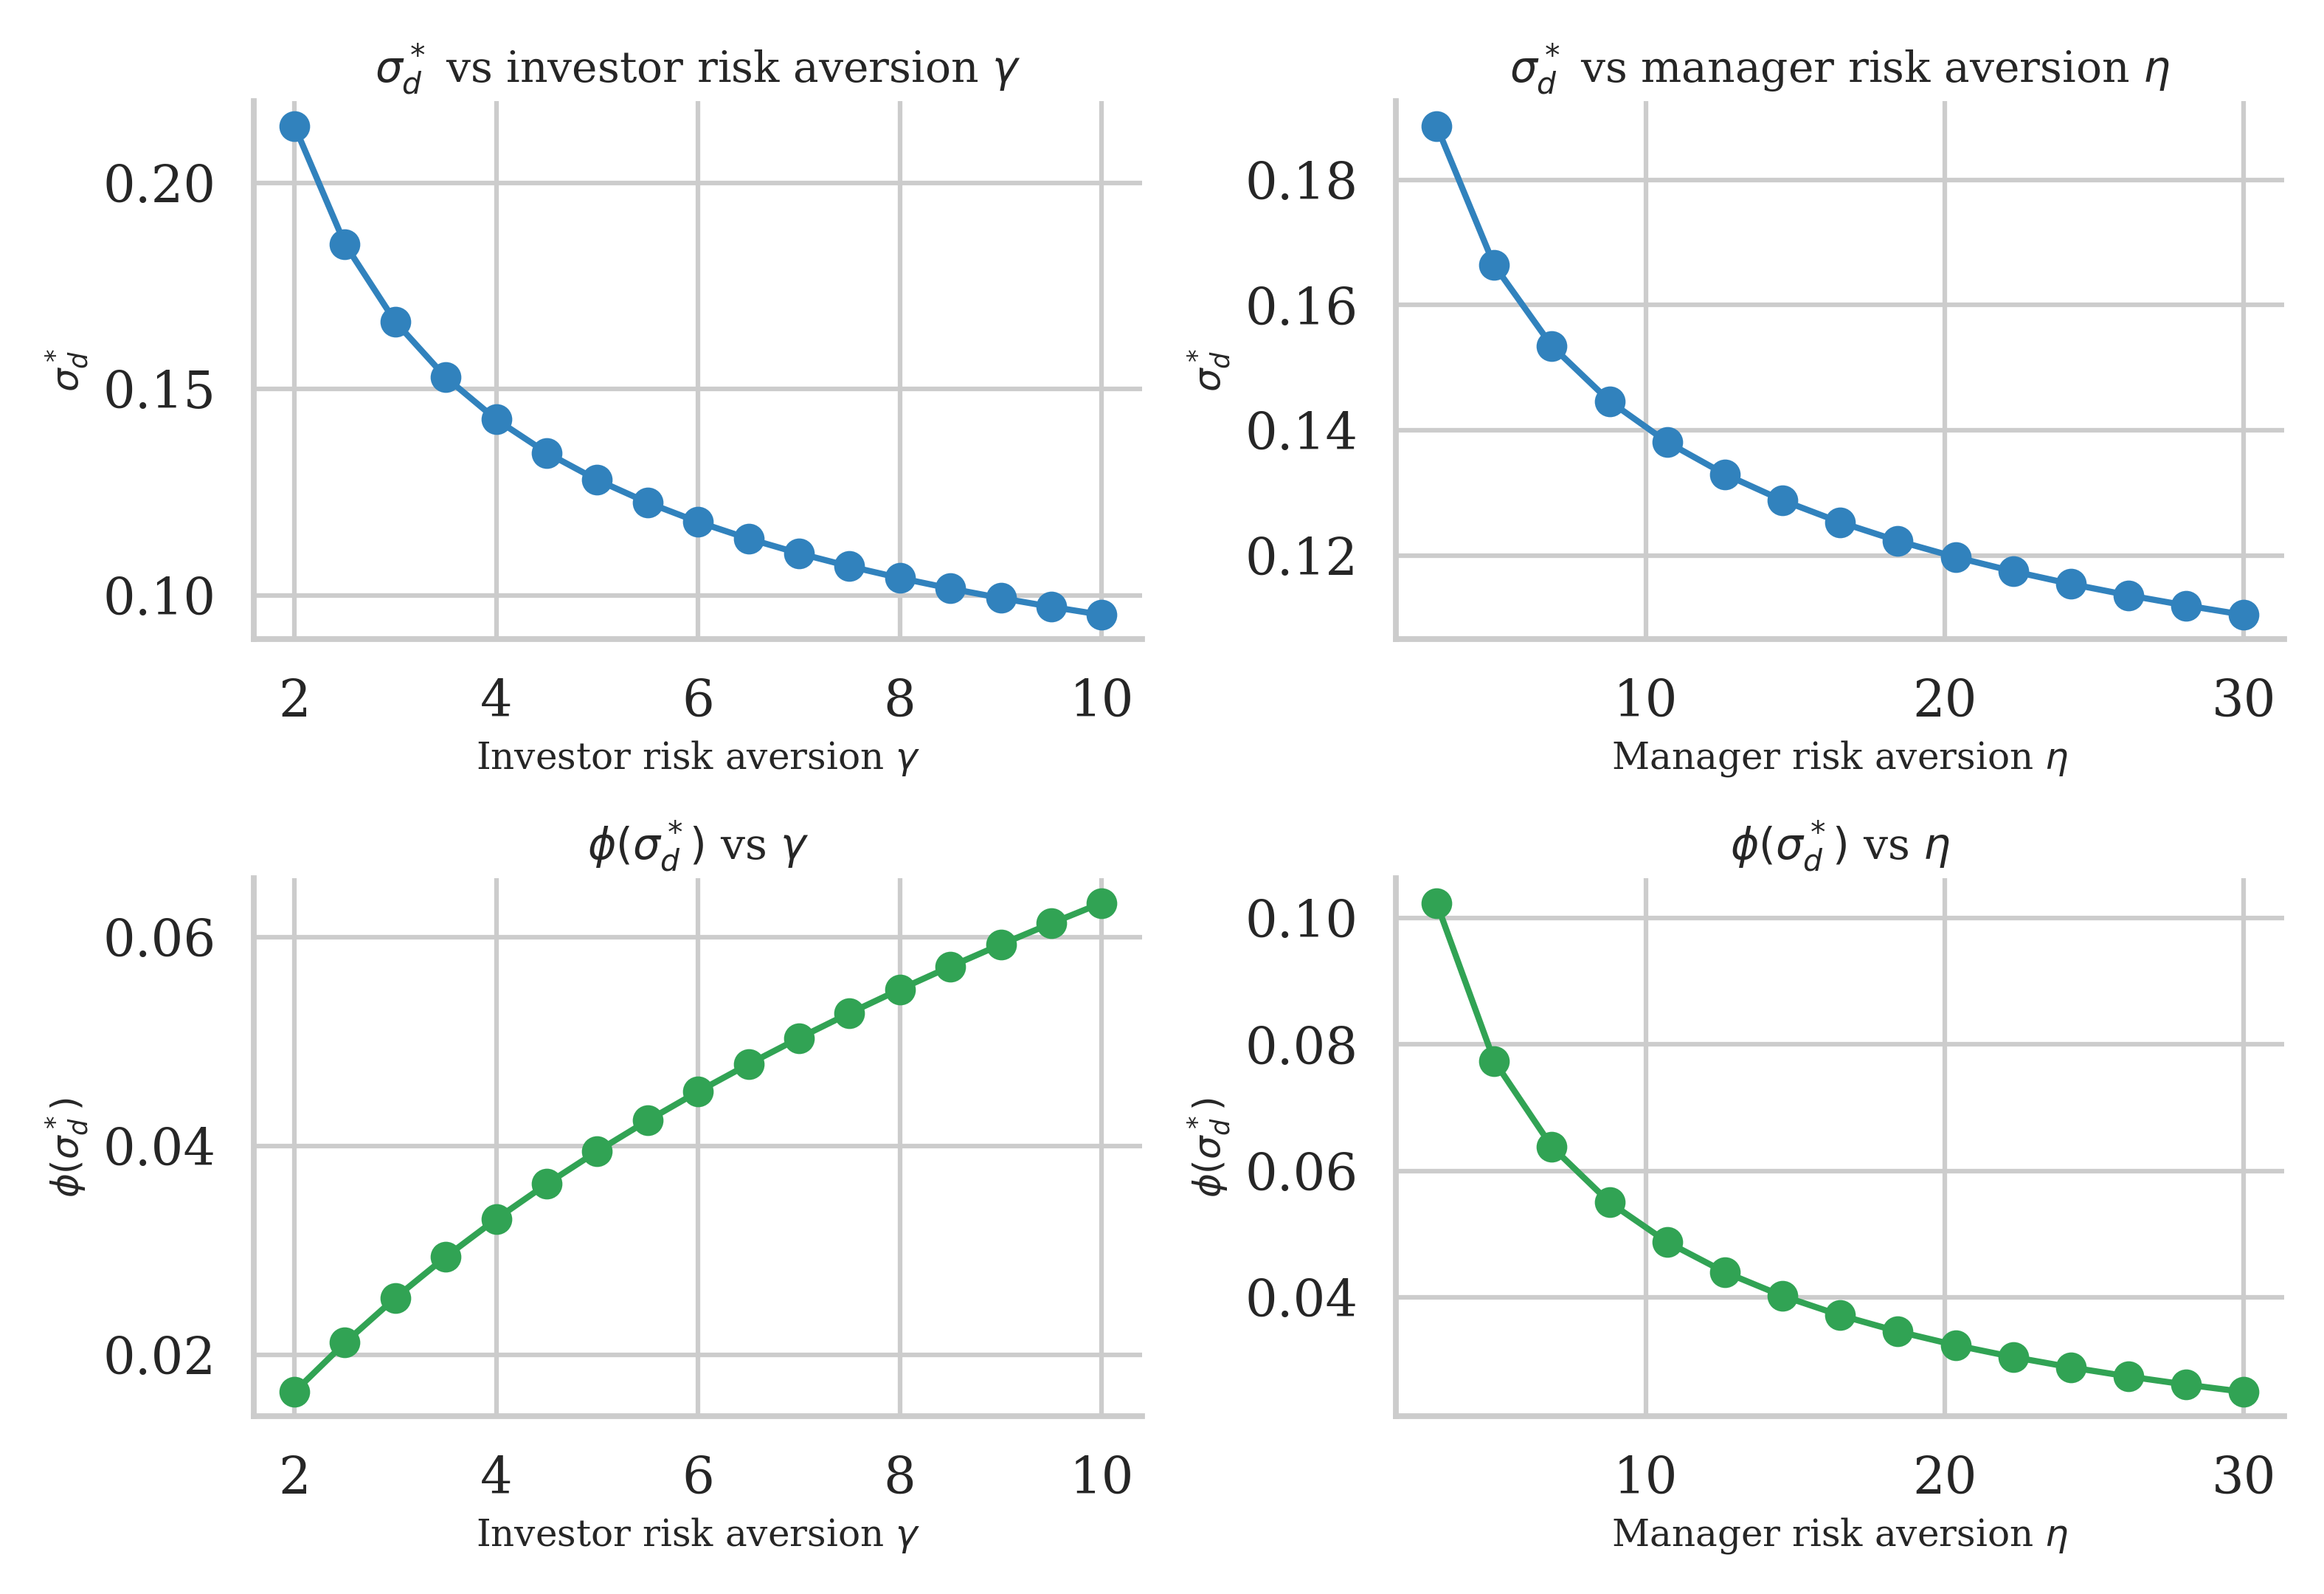
\includegraphics[width=0.95\linewidth]{figures/compstats_risk.png}
    \caption{Risk-aversion effects: optimal target \(\sigma_d^*\) and IC fee at the optimum \(\phi(\sigma_d^*)\) as functions of investor risk aversion \(\gamma\) and manager risk aversion \(\eta\).}
    \fnote{\textit{Note:} Other parameters held at calibration baseline: $\Sharpe=0.35$, $r_f=3.70\%$, $A_0=1$, $f_1=1.5$, $f_2=25$. Left panel varies $\gamma$ with $\eta=15$; right panel varies $\eta$ with $\gamma=5$.}
    \label{fig:comp-risk}
\end{figure}
}{}

\IfFileExists{figures/welfare_comparison.png}{%
\begin{figure}[H]
    \centering
    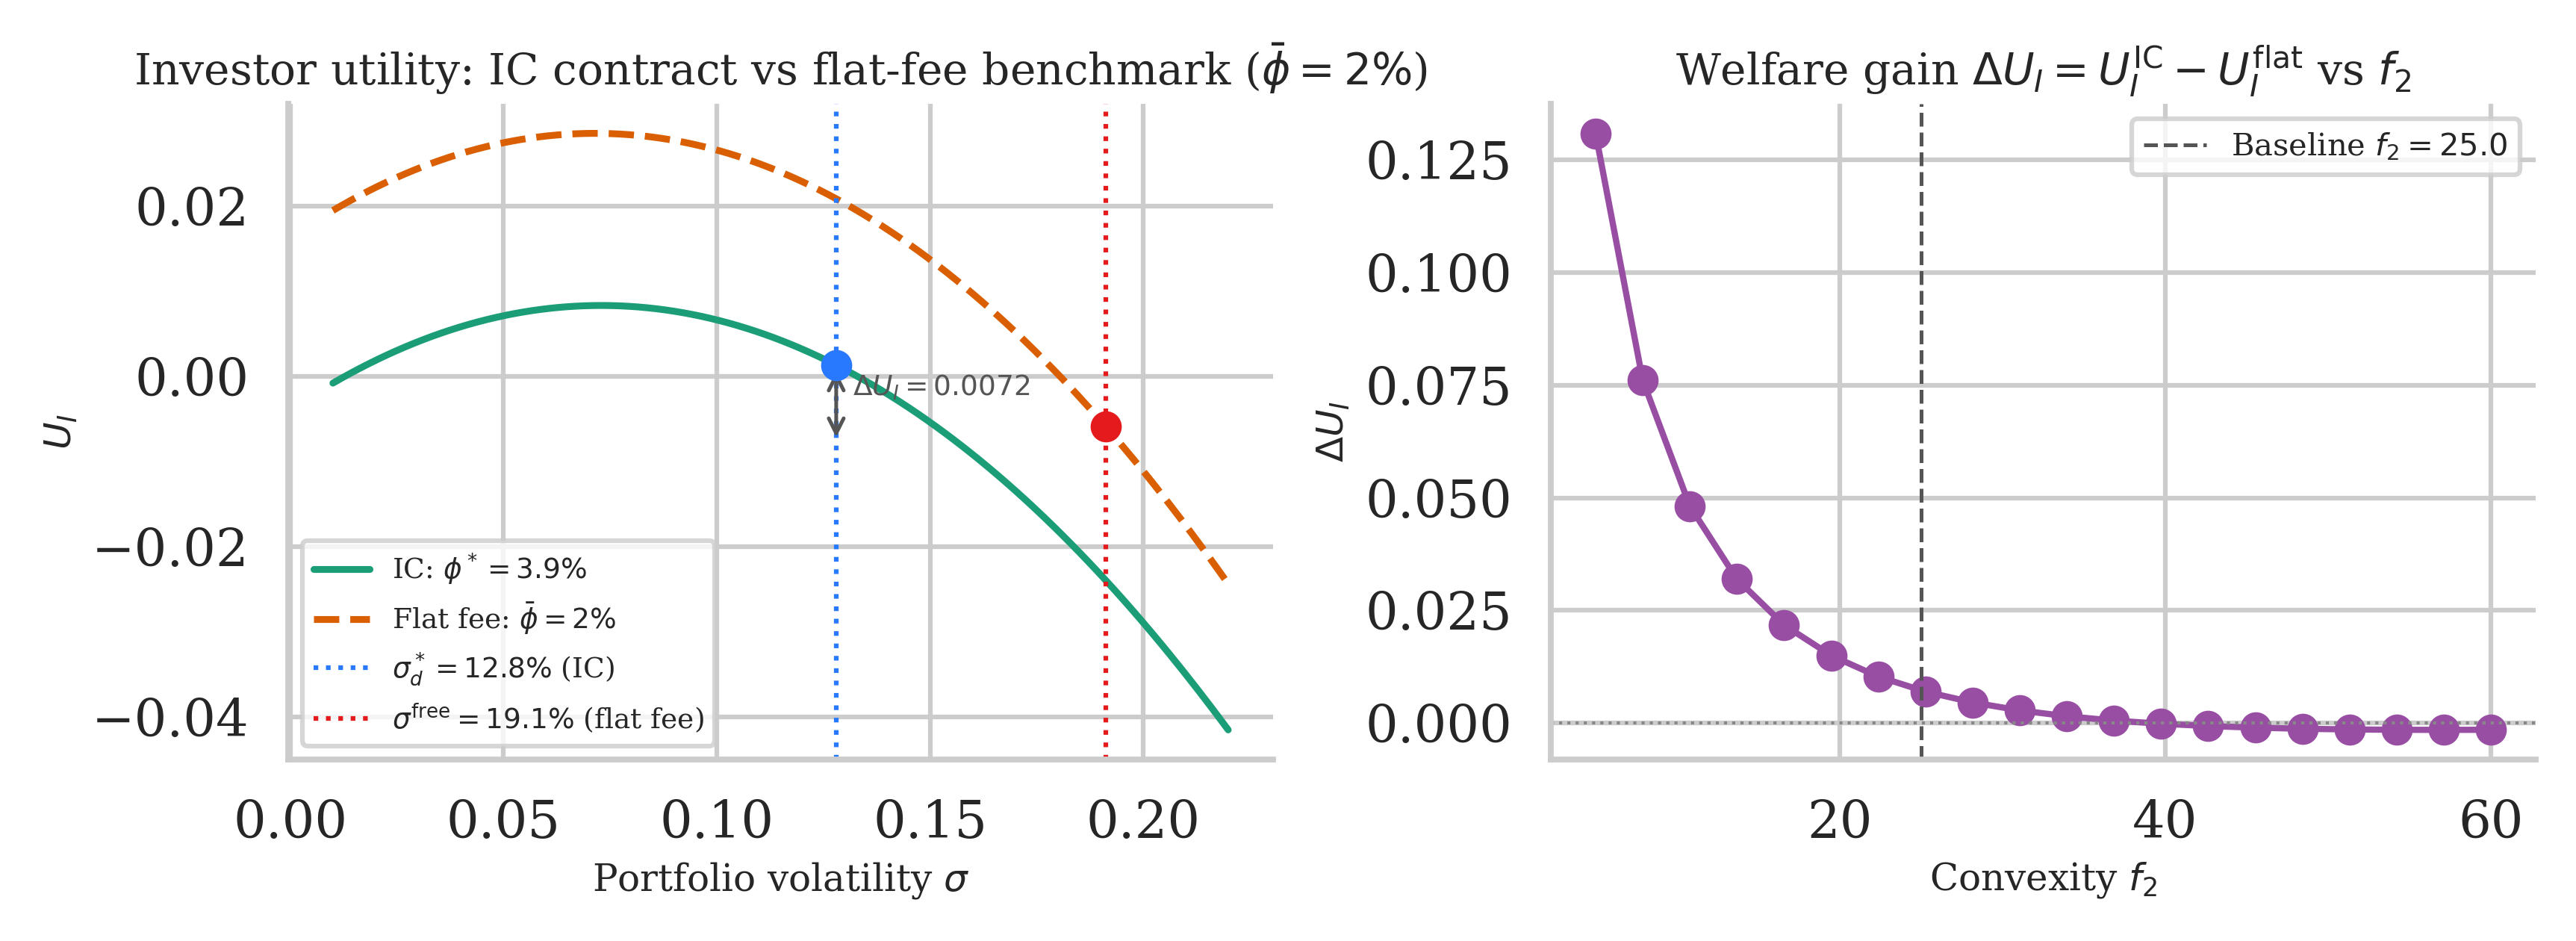
\includegraphics[width=0.95\linewidth]{figures/welfare_comparison.png}
    \caption{Welfare comparison: IC contract vs.\ flat-fee benchmark. The benchmark is a market flat fee $\phi_{\rm mkt}=2\%$; at that fee, the manager freely chooses $\sigma^{\rm free}=\arg\max_\sigma U_M(\sigma;\phi_{\rm mkt})>\sigma_d^*$. \textit{Left panel:} investor utility $U_I(\sigma,\phi)$ as a function of $\sigma$ under the IC fee $\phi^*$ (solid) and the flat fee $\phi_{\rm mkt}$ (dashed); vertical lines mark the IC target $\sigma_d^*$ and the laissez-faire choice $\sigma^{\rm free}$; the shaded gap quantifies the welfare gain $\Delta U_I = U_I(\sigma_d^*,\phi^*)-U_I(\sigma^{\rm free},\phi_{\rm mkt})$. \textit{Right panel:} welfare gain $\Delta U_I$ as a function of the convexity parameter $f_2$, showing that the welfare gain is decreasing in $f_2$: IC enforcement delivers the largest improvement at moderate convexity, and the gain diminishes as convexity increases because the IC fee must fall sharply to maintain incentive alignment.}
    \fnote{\textit{Note:} Calibrated baseline parameters: $\Sharpe=0.35$, $r_f=3.70\%$, $\gamma=5$, $\eta=15$, $A_0=1$, $f_1=1.5$, $f_2=25$.}
    \label{fig:welfare}
\end{figure}
}{}

\IfFileExists{figures/incentive_alignment.png}{%
\begin{figure}[H]
    \centering
    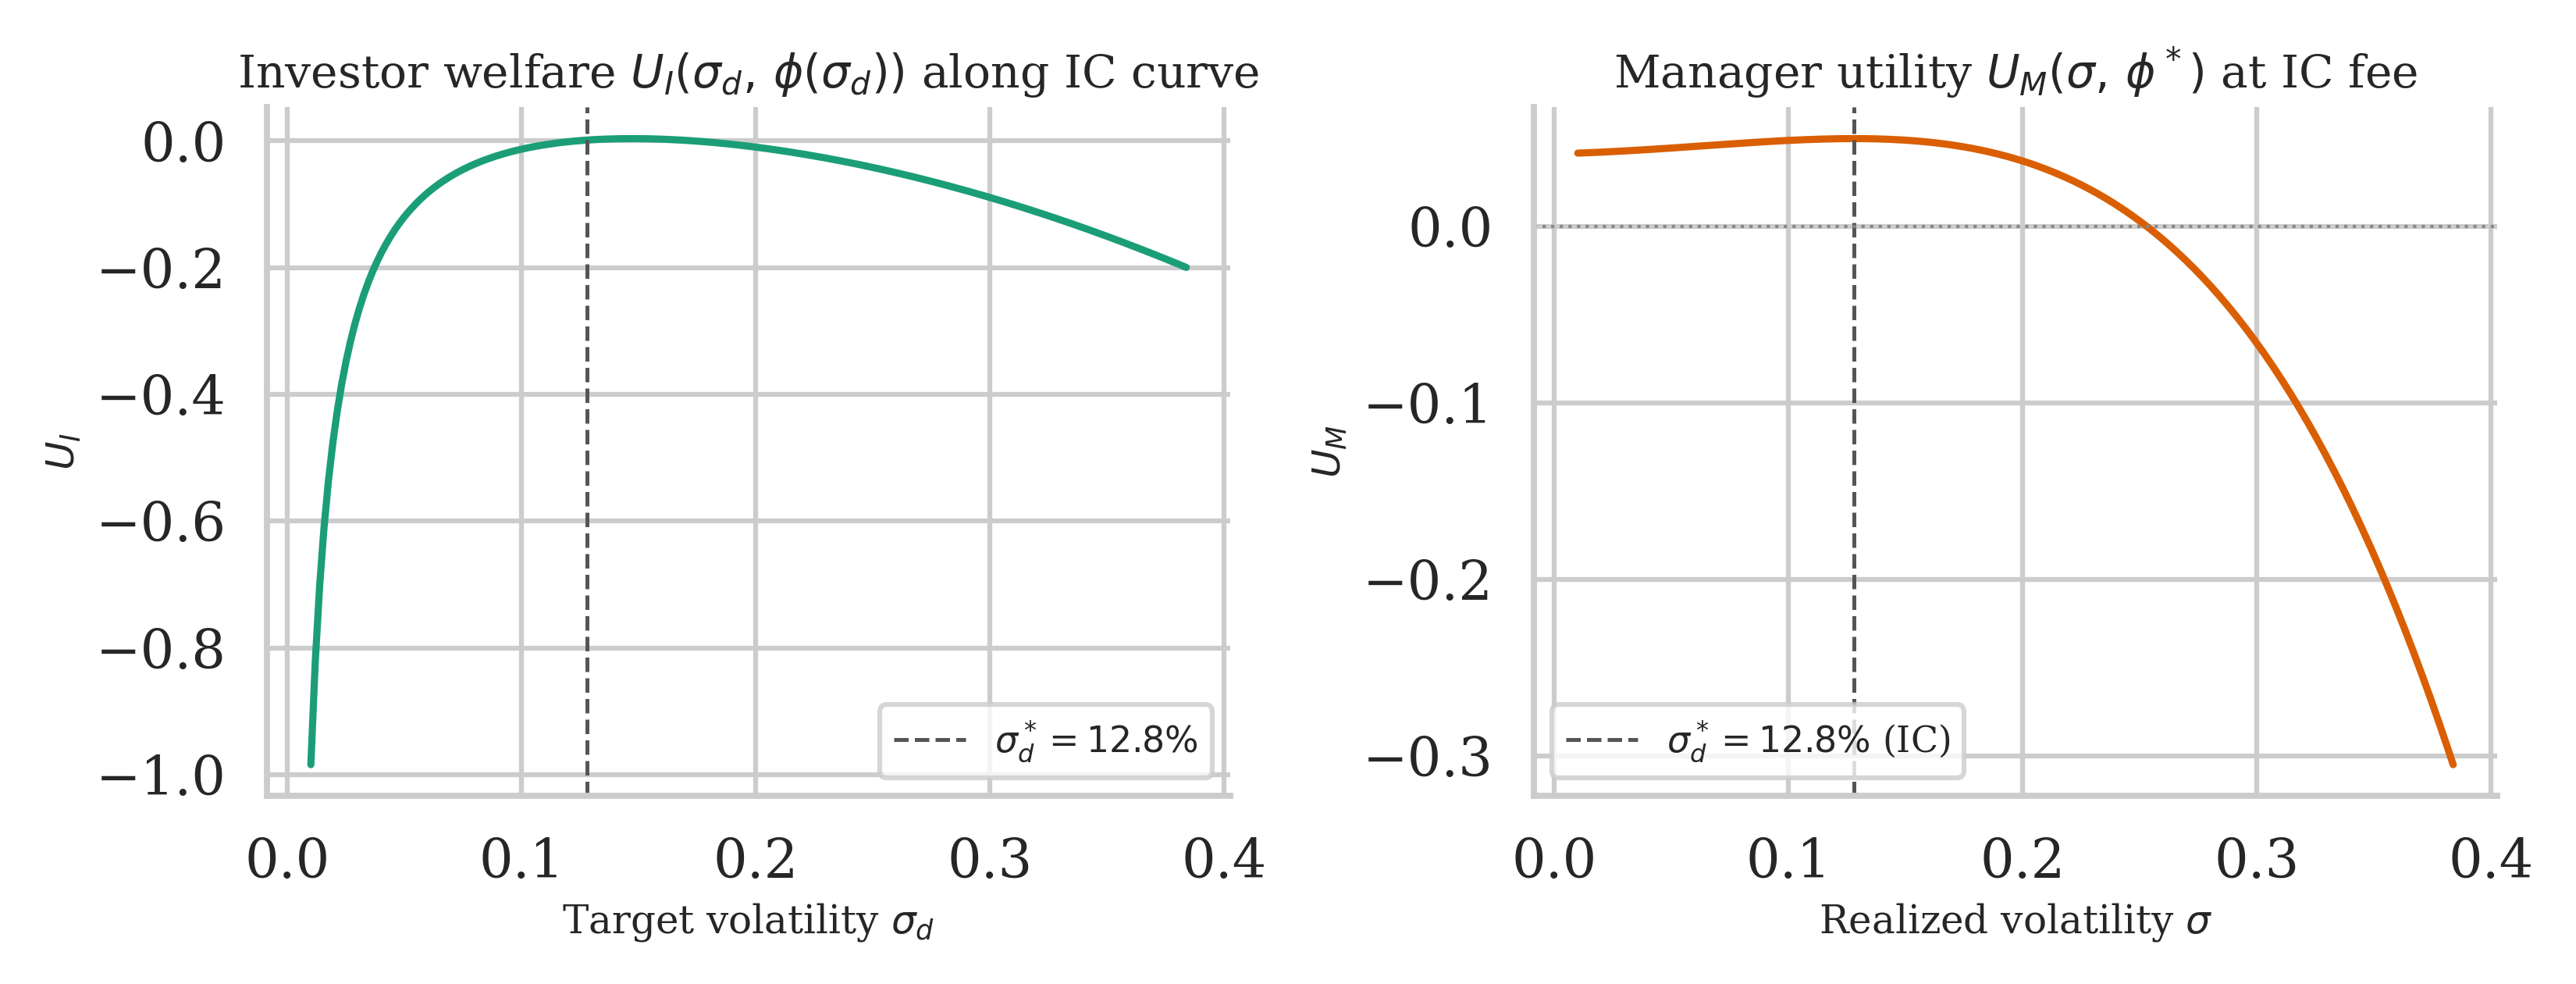
\includegraphics[width=0.95\linewidth]{figures/incentive_alignment.png}
    \caption{Incentive alignment diagnostics under the IC contract. \textit{Left panel:} investor utility $U_I(\sigma_d,\phi(\sigma_d))$ along the IC-feasible frontier as a function of the volatility target $\sigma_d$, with the optimal target $\sigma_d^*$ marked. \textit{Right panel:} manager utility $U_M(\sigma, \phi^*)$ as a function of realized volatility $\sigma$ at fixed IC fee $\phi^*=\phi(\sigma_d^*)$, confirming that the manager's privately optimal choice equals $\sigma_d^*$.}
    \fnote{\textit{Note:} Calibrated baseline parameters: $\Sharpe=0.35$, $r_f=3.70\%$, $\gamma=5$, $\eta=15$, $A_0=1$, $f_1=1.5$, $f_2=25$.}
    \label{fig:incentive-alignment}
\end{figure}
}{}

\IfFileExists{figures/global_ic_verification.png}{%
\begin{figure}[H]
    \centering
    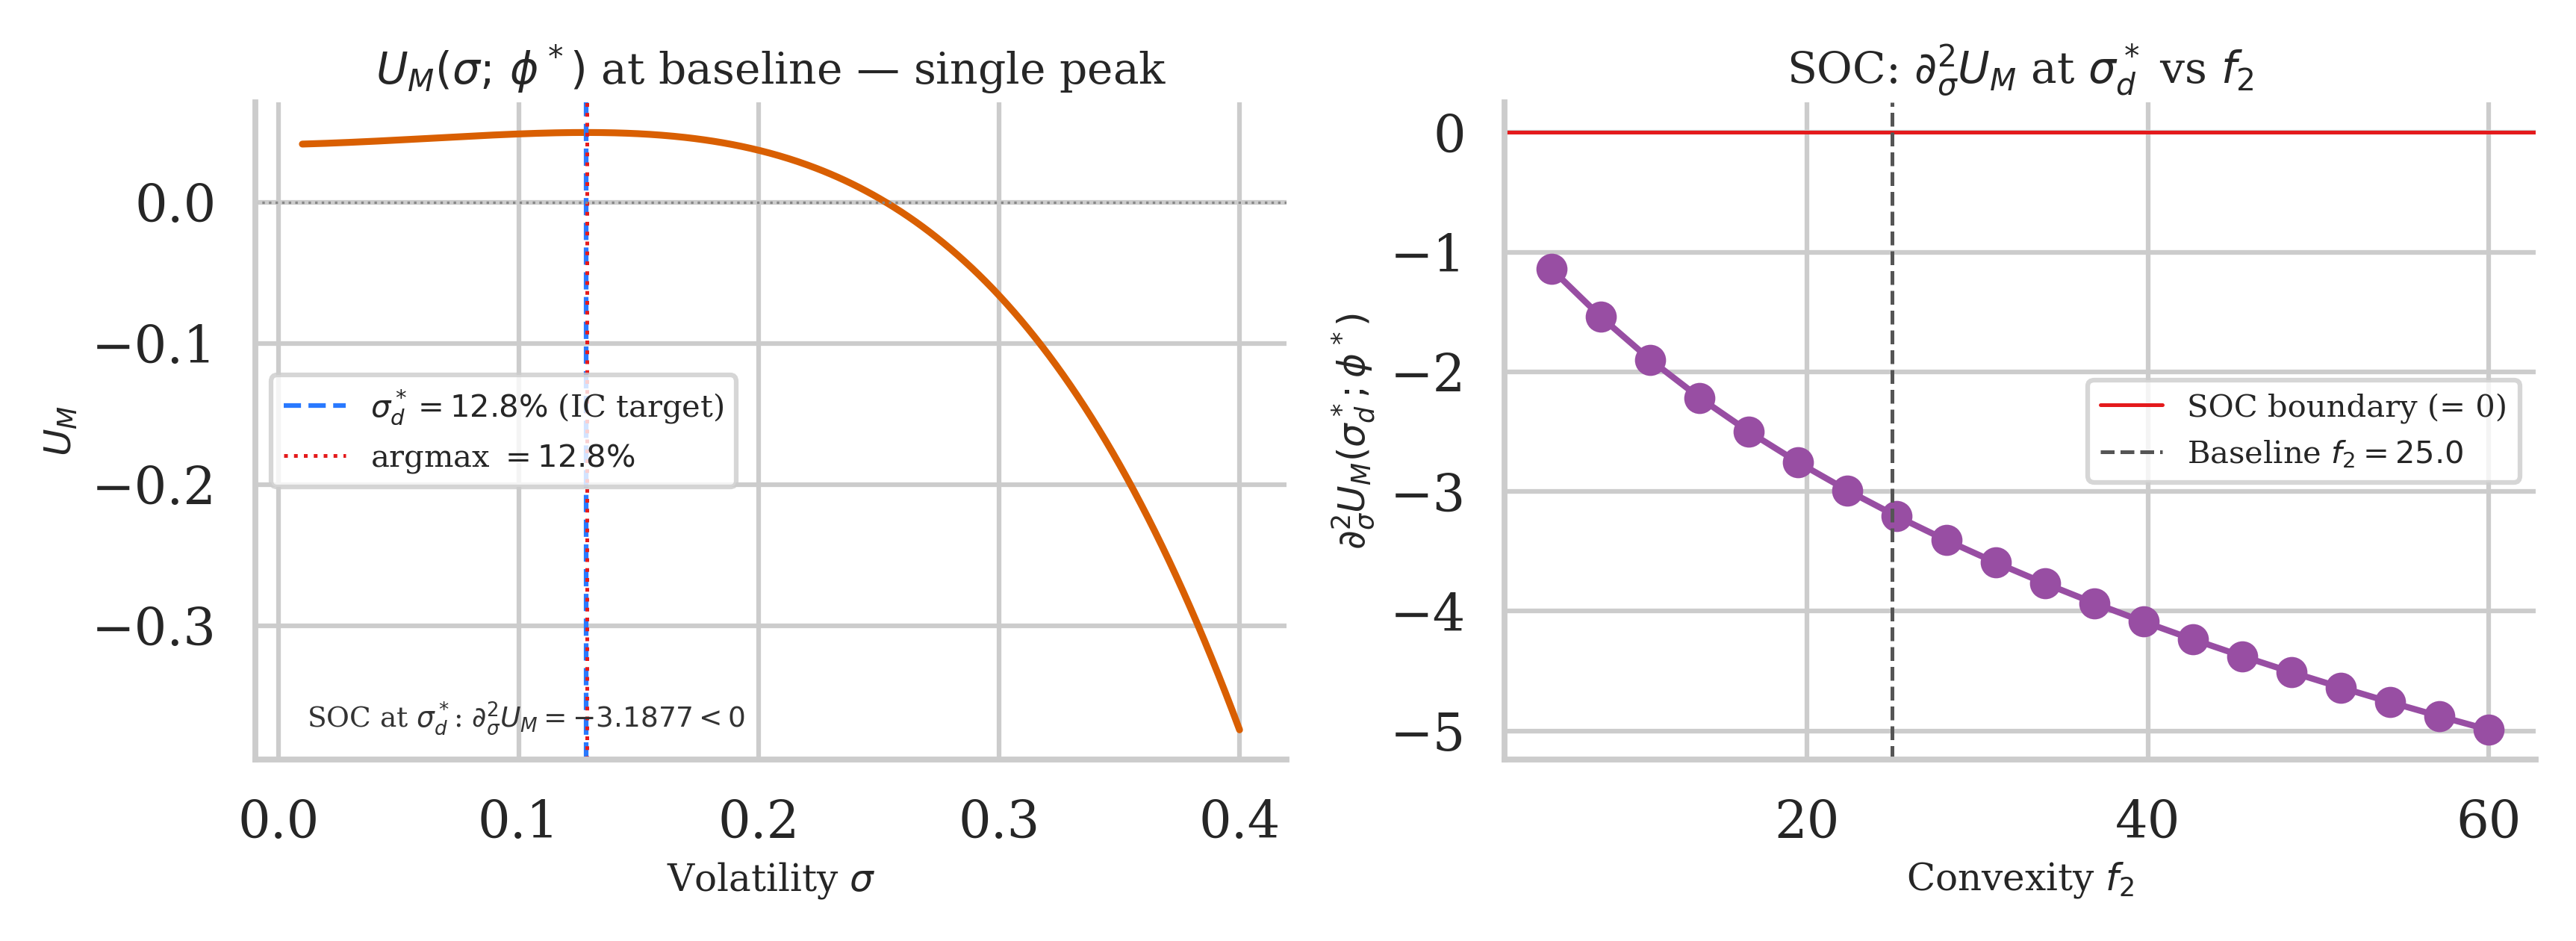
\includegraphics[width=0.95\linewidth]{figures/global_ic_verification.png}
    \caption{Global IC verification. \textit{Left panel:} manager utility $U_M(\sigma;\phi^*)$ over the full range $\sigma\in[0.01,0.40]$ at the baseline IC fee $\phi^*$, confirming a unique maximum at $\sigma_d^*$ (dashed line); the argmax coincides with the IC target to three decimal places. The second-order condition $\partial^2_\sigma U_M(\sigma_d^*;\phi^*)<0$ (reported in panel label) holds strictly. \textit{Right panel:} SOC value $\partial^2_\sigma U_M$ evaluated at $(\sigma_d^*,\phi^*)$ across the $f_2$ sweep; all values are negative, confirming the SOC holds throughout the calibrated parameter grid.}
    \fnote{\textit{Note:} Calibrated baseline parameters: $\Sharpe=0.35$, $r_f=3.70\%$, $\gamma=5$, $\eta=15$, $A_0=1$, $f_1=1.5$, $f_2=25$. Right panel sweeps $f_2\in[5,60]$ with all other parameters at baseline.}
    \label{fig:global-ic}
\end{figure}
}{}

\IfFileExists{figures/affine_approx_quality.png}{%
\begin{figure}[H]
    \centering
    
\includegraphics[width=0.85\linewidth]{figures/affine_approx_quality.png}
    \caption{Quality of the affine approximation: average absolute error (in percentage points) between the exact IC fee \(\phi(\sigma_d)\) and its linear approximation. For each convexity parameter \(f_2\), the approximation is centered at the optimal target \(\sigma_d^*\) and evaluated within \(\pm 5\%\) of that target.}
    \fnote{\textit{Note:} Other parameters held at calibration baseline: $\Sharpe=0.35$, $r_f=3.70\%$, $\gamma=5$, $\eta=15$, $A_0=1$, $f_1=1.5$.}
    \label{fig:affine-approx}
\end{figure}
}{}
